\documentclass{homeworg}

\title{Architectural Decision Document:\\\textbf{Credit Card Churn Prediction}}
\author{Alif Sussardi}
\usepackage{hyperref}
\usepackage[section]{placeins}
\usepackage{float}
\usepackage{array}
\hypersetup{
    colorlinks=true,
    linkcolor=blue,
    filecolor=blue,      
    urlcolor=blue,
}
\begin{document}
\graphicspath{ {./figure/} }
\maketitle

\section{Overview}
Credit Card Churn Prediction was carried out as follow:
\begin{enumerate}
    \item Dataset: Use and Case
    \item Exploratory Data Analysis
    \item Extract, Transform and Load
    \item Feature Creation
    \item Model Definition
    \item Model Training
    \item Model Evaluation
    \item Model Deployment
\end{enumerate}

\section{Dataset and Use Case}
\subsection{Data Choice and Use Case}
The purpose of this Project is to classify the churn of Credit Card customer given several parameters as shown in Column Name.
The data was obtained from Kaggle: \href{https://www.kaggle.com/sakshigoyal7/credit-card-customers}{Churn Data}.
As a company who issue credit card, it is important that we know whether customer will be able to continue their transactions (not defaulted) and keep using our service. The pre-registered features such as Gender, Income Category, Total Relationship Count, can be an indicator whether a customer will be able to sustain our service. 
However, here, I will use all the parameters which are available for the customer that has already registered to see what type of customer will sustain, therefore once we spot a customer with such characteristic, we can reach to them, send them offer to keep using our services.
The parameters that are available in the data is as follow:

\begin{enumerate}
    \item CLIENTNUM = Client number. Unique identifier for the customer holding the account.
    \item Attrition Flag = THIS IS THE TARGET PARAMETER.
    \item Customer Age.
    \item Gender = Demographic variable - M=Male, F=Female.
    \item Dependent count = Demographic variable - Number of dependents.
    \item Education Level.
    \item Marital Status.
    \item Income Category = Annual Income Category of the account holder (< 40K, 40K - 60K,  60K - 80K,  80K - 120K, > 120K, Unknown).
    \item Card Category = Product Variable - Type of Card (Blue, Silver, Gold, Platinum).
    \item Months on Book = Period of relationship with bank.
    \item Total Relationship Count = Total no. of products held by the customer.
    \item Months Inactive 12 mon = No. of months inactive in the last 12 months.
    \item Contacts Count 12 mon = No. of Contacts in the last 12 months.
    \item Credit Limit.
    \item Total Revolving Bal = Total Revolving Balance on the Credit Card.
    \item Avg Open To Buy = Open to Buy Credit Line (Average of last 12 months).
    \item Total Amt Chng Q4-Q1 = Change in Transaction Amount (Q4 over Q1).
    \item Total Trans Amt = Total Transaction Amount (Last 12 months).
    \item Total Trans Ct = Total Transaction Count (Last 12 months).
    \item Total Ct Chg Q4-Q1 = Change in Transaction Count (Q4 over Q1)
    \item Avg Utilization Ratio = Average Card Utilization Ratio
\end{enumerate}

\subsection{Justification}
This data was chosen because it is interesting and important to determine which feature and which Machine Learning or Neural Network are the best in predicting the churn.
\section{Exploratory Data Analysis}
From this exploratory data analysis, we can see how the data spread, and whether some algorithm might not be appropriate. 
\subsection{Correlation Matrix}
From the correlation matrix below we can identify which features are the most important to explain the Attrition Flag. 
\begin{figure}[!h]
    \centering
    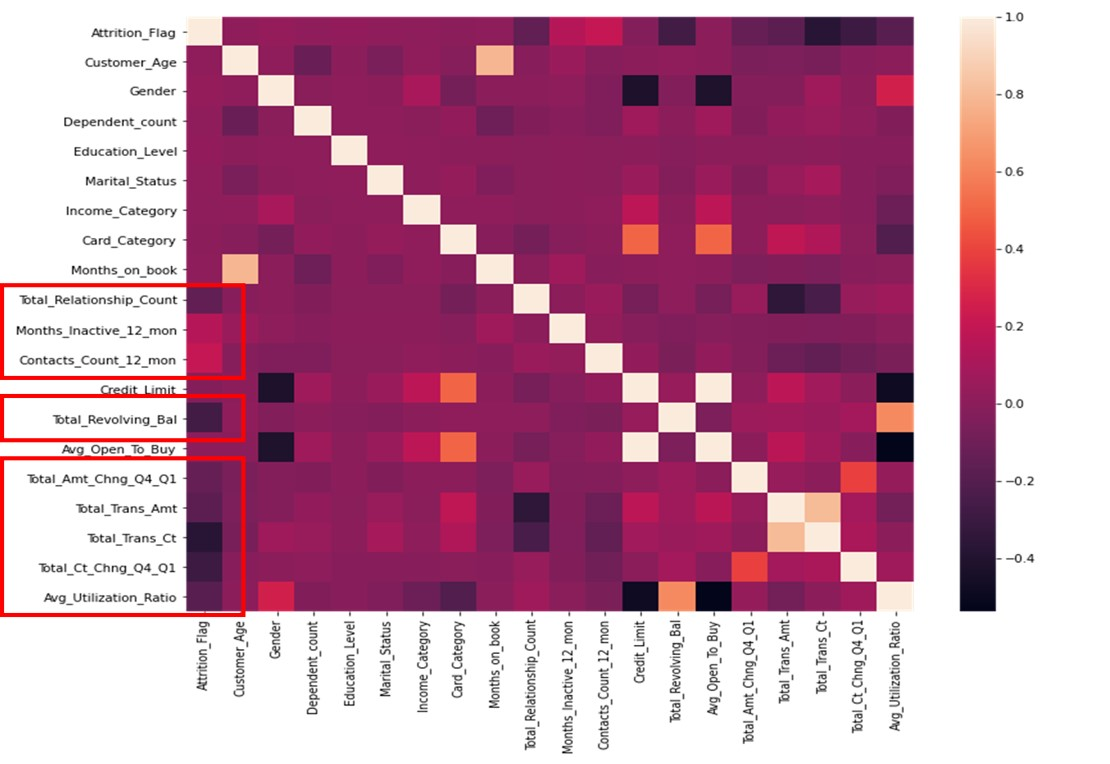
\includegraphics[scale=0.9]{figure/CM_correlation_matrixs.jpg}
    \caption{Correlation matrix}
    \label{fig:cormat}
\end{figure}
From the Figure \ref{fig:cormat} we can see that the Total Transaction, Total Count of Change Q4-Q1, Total Revolving Balance, Contact count, Total Transaction Amount are correlated to the Attrition Flag. Lets see What they are looks like later. 
For now We can see how these data behaved.
The features, however, can be divided into Categorical and Numerical. And will be shown as follow. (Only important data are shown) \newpage
\subsection{Features Outlook}
\subsubsection{Attrition Flag}
It can be seen that the Attrition Flag distribution is not great, with the count of Existed cases 5 times the Attrited cases. This type of data might be bad for making a model as it will introduce bias towards the Existed, means the machine will predict Existed customer better than the Attrited due to having more training.
\begin{figure}[H]
    \centering
    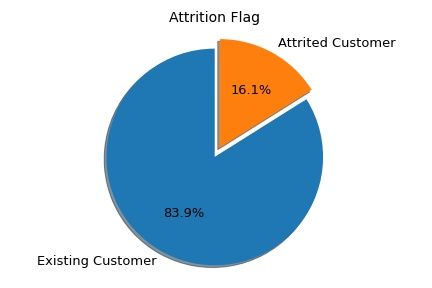
\includegraphics[scale=0.7]{figure/PC_Attrition.jpg}
    \caption{Attrition Flag}
    \label{fig:attrition}
\end{figure}
\par
\subsubsection{Total Transaction Count}
The Total transaction count data is not normally distributed, which is not good if we want to use standard scaler. 
It looks like there are 3 main groups around 40, 80 and 110 transaction amount.
\begin{figure}[H]
    \centering
    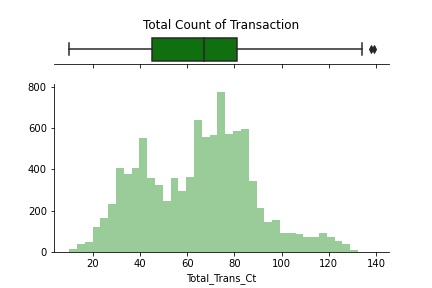
\includegraphics[scale=0.7]{figure/HG_Transaction_counts.jpg}
    \caption{Gender Ratio}
    \label{fig:transcount}
\end{figure}
\par
\subsubsection{Average Utilization Ratio}
The Average utilization ratio is also not normally distributed, with most of the user not using their card! This type of behaviour is also not good for StandardScaler scaling model.
\begin{figure}[H]
    \centering
    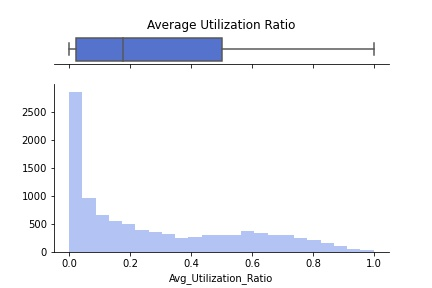
\includegraphics[scale=0.7]{figure/HG_Util_ratio.jpg}
    \caption{Utilization Ratio}
    \label{fig:utilratio}
\end{figure}
\par
\subsubsection{Change from Q1 to Q4}
The Total Amount of change is normally distributed, with a small kurtosis on the right hand side of the graph.
\begin{figure}[H]
    \centering
    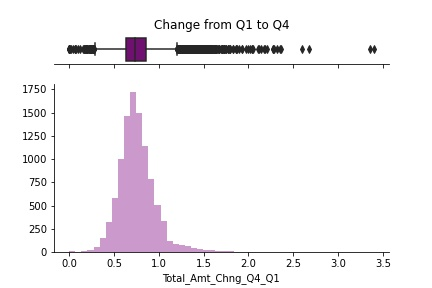
\includegraphics[scale=0.7]{figure/HG_TotalChangeQ1-Q4.jpg}
    \caption{Total Change Q1-Q4}
    \label{fig:Q4Q1Change}
\end{figure}
\par
\subsubsection{Total Relationship}
The total number of relationship does not seem like have any pattern. But it can be seen that most of the customer has at least 3 relationships, meaning they have several cards at once.
\begin{figure}[H]
    \centering
    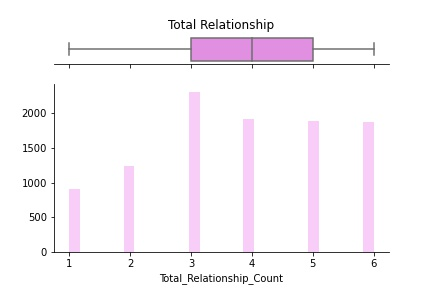
\includegraphics[scale=0.7]{figure/HG_Total_relationship.jpg}
    \caption{Total relationship}
    \label{fig:totalrelationship}
\end{figure}
\par
\subsubsection{Total Transaction Amount}
It can be seen clearly that there are at least 4 groups. One at 2000 USD,at 4500 USD, 8000 USD and 15000 USD. This data cannot be scaled using StandardScaler as well.
\begin{figure}[H]
    \centering
    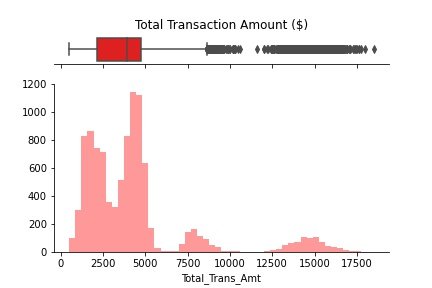
\includegraphics[scale=0.7]{figure/HG_Total_transaction.jpg}
    \caption{Total Transaction}
    \label{fig:totaltransaction}
\end{figure}
\par
\subsubsection{Contact Count}
Number of contact in 12 months are evenly distributed between 2 and 3. Meaning that, the customer mostly contacting our Credit Card company 2 or 3 times. Better be preparing for that Customer Service Call! If we want to add more customer!
\begin{figure}[H]
    \centering
    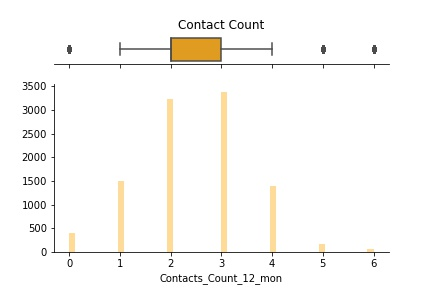
\includegraphics[scale=0.7]{figure/HG_Contacts_count.jpg}
    \caption{Contact Count}
    \label{fig:contactcount}
\end{figure}
\par
\subsubsection{Total Revolving Balance}
This quite strange, because most of the people does not have any balance, while the rest of the people has average of about 1500 USD with large variation from 500 to 2500, but the affluent customer are second to the one without balance.
\begin{figure}[H]
    \centering
    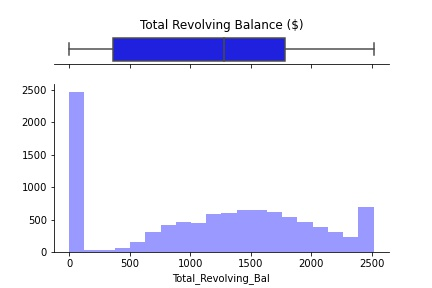
\includegraphics[scale=0.7]{figure/HG_Total_rev_balance.jpg}
    \caption{Total Revolving Balance}
    \label{fig:revbal}
\end{figure}
\par
\subsubsection{Months Inactivity}
This is the weirdest amongst all. Lets take a look, there are seems to be a cut at 3 months inactivity here. Is it that marketing guy again, who did some campaign 3 months ago? or most customer just cancel their account after 3 months?
\begin{figure}[H]
    \centering
    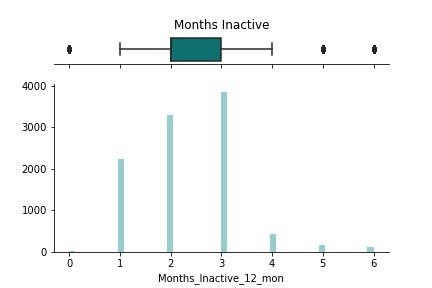
\includegraphics[scale=0.7]{figure/HG_Month_inactive.jpg}
    \caption{Month Inactivity}
    \label{fig:inactivity}
\end{figure}



\section{Extract, Transform \& Load (ETL)}
\subsection{Technology Choice}
All operations in this data analysis and modeling were done in \textbf{Jupyter Notebook}, using \textbf{Google Cloud Server}.\\
The data were imported from the BankChurner.csv file downloaded from kaggle, as mentioned in the introduction.\par

\subsection{Feature Creation}
All data transformation were done using \textbf{pandas} and \textbf{numpy} as they are the most commonly used tools and easy to use. 
The Categorical data were transformed with \textbf{pandas} \textbf{factorize} as follow:
\begin{figure}[H]
    \centering
    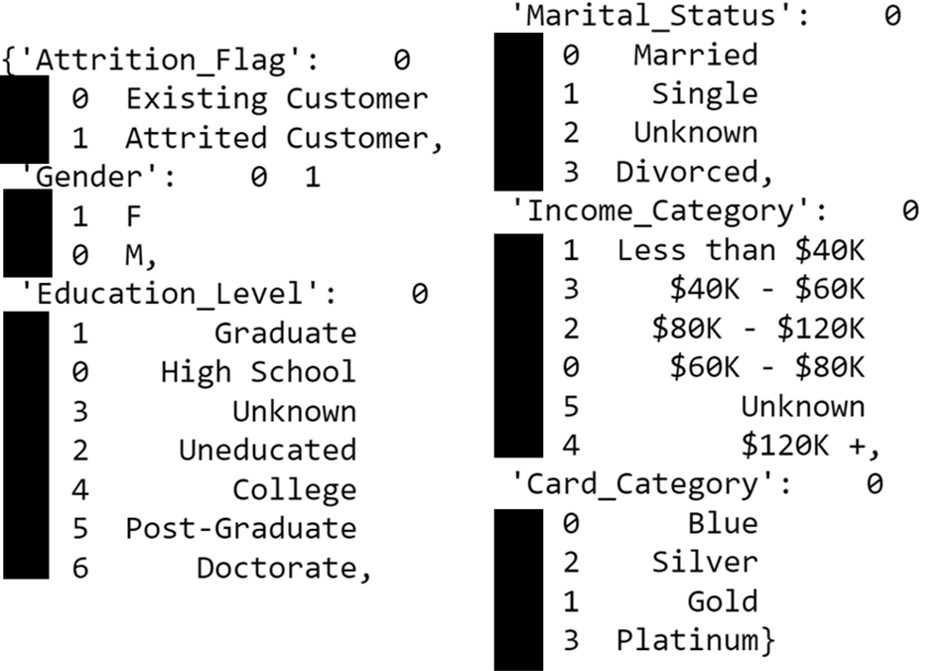
\includegraphics[scale=0.7]{figure/Categorization.jpg}
    \caption{Categorization}
    \label{fig:category}
\end{figure}
\par

\subsection{Data splitting and Synthesis}
The date were then transformed into array with \textbf{numpy} and scaled using \textbf{sklearn} \textbf{MinMaxScaler}.\\
After scaled, the data then split into 80\% train and 20\% test. Later the train data split again into train (80\%) and validation (20\%) data. This also means that the test data consist of 20\%, the train is 64\% and 16\% of the validation from the total data provided.\\
\begin{figure}[H]
    \centering
    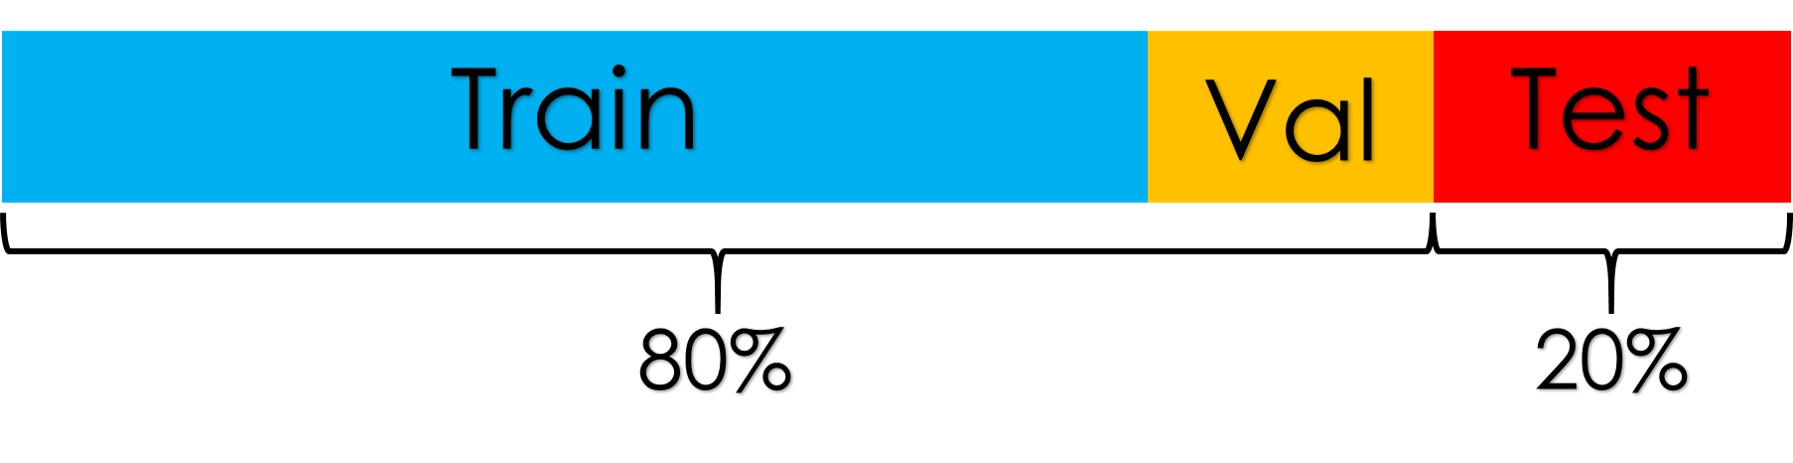
\includegraphics[scale=0.4]{figure/traintest.jpg}
    \caption{Train, Validation \& Test data}
    \label{fig:traintest}
\end{figure}
\par
Data were synthesized using \textbf{imbalanced-learn} \textbf{SMOTE} algorithm on the original data to obtain the same number of Attrited and Existed data:
\begin{figure}[H]
    \centering
    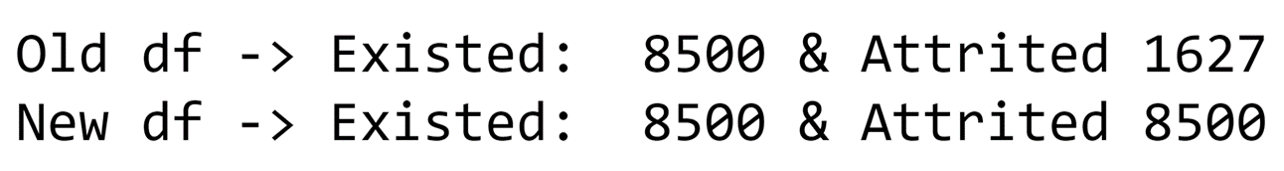
\includegraphics[scale=0.5]{figure/SMOTE.png}
    \caption{Old \& New Data}
    \label{fig:oldnewdata}
\end{figure}

\subsection{Justification}
\textbf{Jupyter Notebook} were used as it is easy and can be run line-by-line in a separate server. In fact, the server that I was using was \textbf{Google Cloud Server}, as it is significantly cheaper (three month promos with \$300 balance) without limitation of CPU's usage or power, compared to IBM Watson.\\
\textbf{Pandas factorize} was used as opposed to \textbf{sklearn one-hot-encoder} as I want to do modeling fast, in a sacrifice of data clarity, the factorization or label encoder will introduced hierarchial bias on each category, but it will have significantly smaller feature than onehot encoder.\\
Test data of 20\% was chosen as I think 20\% is enough number to reveal whether the model will overfit or not.\\
\textbf{sklearn MinMaxScaler} was used to normalize the data as we can see from the Exploratory data analysis that the distribution are not normal/Gaussian, using StandardScaler (data divided by standard deviation) algorithm will make it bad, as the standard deviation cannot reflect the spread of the data from the mean.
\section{Model Definition}
\subsection{Machine Learning}
The supervised machine learning classifiers were used, including:
\begin{enumerate}
    \item \textbf{Random Forest Classifier} by \textbf{scikit-learn},
    \item \textbf{Logistic Regression} by \textbf{scikit-learn},
    \item \textbf{XGBoost Classifier} from \textbf{xgboost} package,
    \item \textbf{Light Gradient Boosting Machine} from \textbf{lightgbm} package.
\end{enumerate}
Both original and synthesized data were fed into the machine learning on their default parameters.
\subsection{Neural Network}
Deep learning were carried out using \textbf{tensorflow keras} machine.
\subsubsection{Long Neural Network}
The long Neural Network is a Sequential neural network, consisting 6 hidden layers, as follow:
\begin{figure}[H]
    \centering
    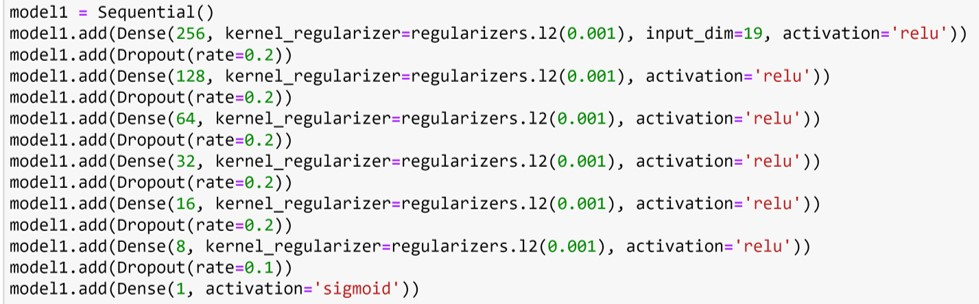
\includegraphics[scale=0.6]{figure/Long NN.jpg}
    \caption{Long Neural Network}
    \label{fig:longNN}
\end{figure}

\subsection{Wide Neural Network}
The wide neural network is also Sequential neural network, consisting of only 3 hidden layer, but with significantly more neuron, as shown below:
\begin{figure}[H]
    \centering
    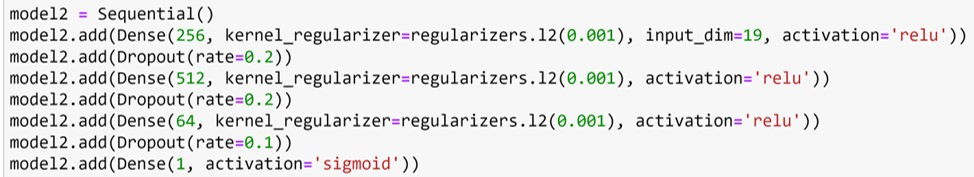
\includegraphics[scale=0.6]{figure/Wide NN.jpg}
    \caption{Wide Neural Network}
    \label{fig:wideNN}
\end{figure}

\subsection{Justification}
Random Forest and Logistic regression were chose as they are the most common machine learning, and also simplest. On the other hand, the XGBoost and LGBM were chosen as they are slightly more advanced.\\
The Deep learning were varied for Wide and Long Neural Network to compare which one is the more effective algorithms.

\section{Model Training}
\subsection{Machine Learning}
Machine Learning algorithms were trained using original train data and synthesized data using SMOTE.
\subsection{Deep Learning}
Binary Crossentropy were used to calculate the loss, using ADAM optimizer.
\begin{figure}[H]
    \centering
    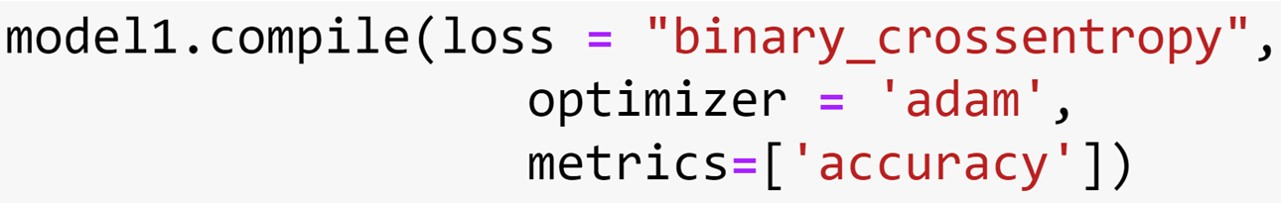
\includegraphics[scale=0.5]{figure/compile.jpg}
    \caption{Compile}
    \label{fig:compile}
\end{figure}
The model were trained using scaled data, both the original and after synthesised using SMOTE, and validation data were used for the validation, with 150 epochs.
\begin{figure}[H]
    \centering
    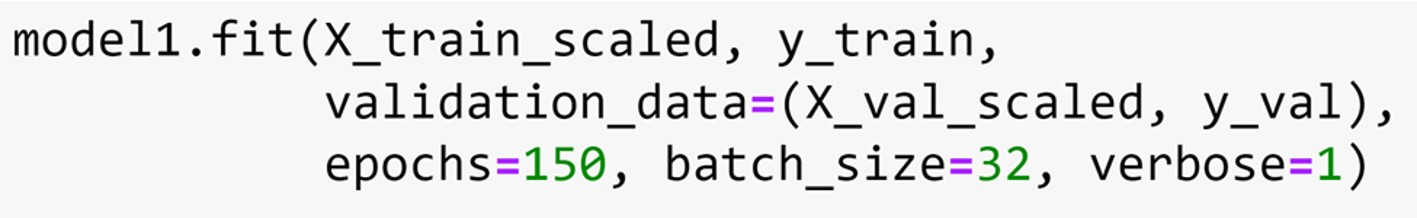
\includegraphics[scale=0.5]{figure/fit.jpg}
    \caption{Fit}
    \label{fig:fit}
\end{figure}

\subsection{Justification}
Algorighm were trained using Train and evaluated using Validation data (Original and SMOTEd) to avoid over-fitting.
Binary Crossentropy were chosen as the target or predicted feature is binary, and it takes into account for both Attrited and Existed.\\
ADAM was used as it is the fastest optimizer with reasonable ability to reach least gradient with avoiding local minimum. It was excellent!\\
150 epochs were chosen as it was thought that after 150 cycle, the accuracy or loss will converge.

\section{Model Evaluation}
All Machine Learning models were evaluated using cross validation method on its training data with 5 cross validation batches.
Both Machine Learning and Deep Learning methods were also evaluated using test data to see its evaluations scores (Accuracy, F1 and Recall).

\subsection{Machine Learning Confusion Matrix}
By comparing the two sets of Original and SMOTEd data, we can see clearly that the proportion of correct guess are better in the SMOTEd Data.
\begin{figure}[H]
    \centering
    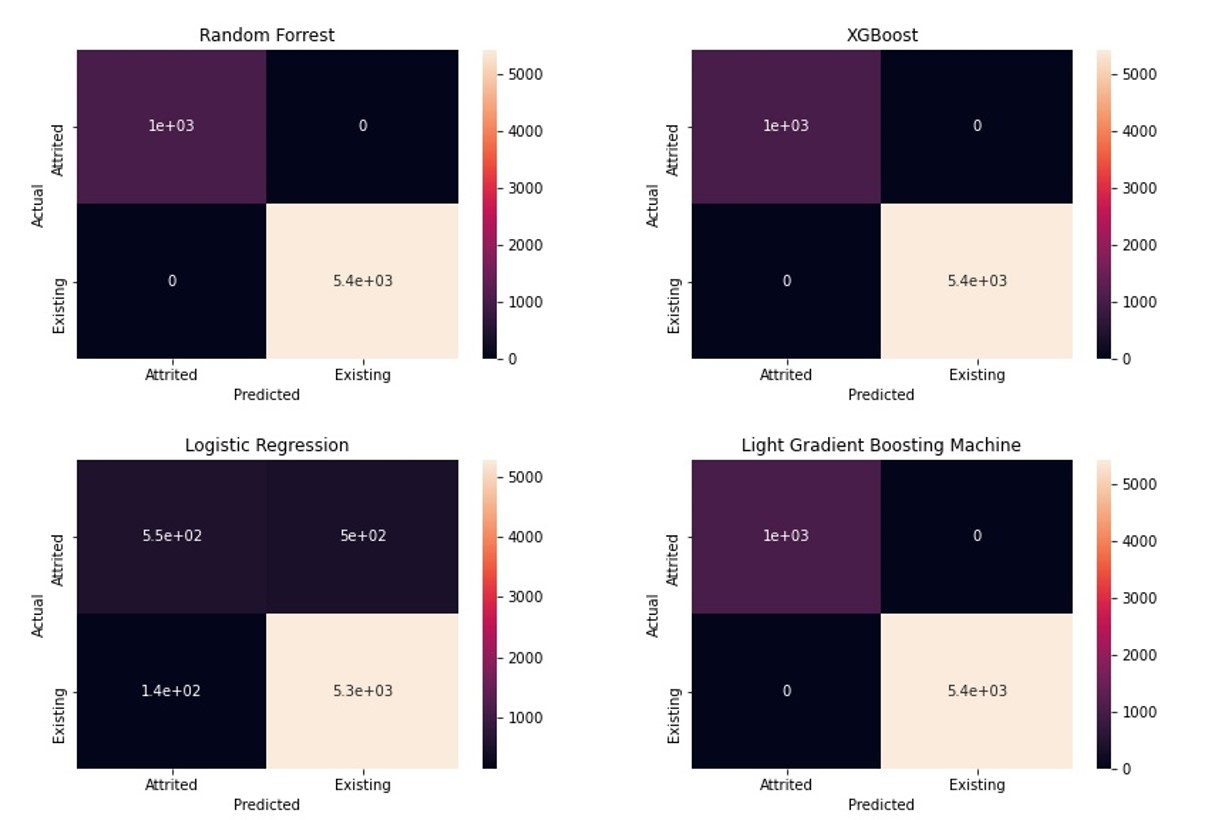
\includegraphics[scale=0.6]{figure/ML No SMOTE.jpg}
    \caption{Confusion matrix: Machine Learning Original Data}
    \label{fig:MLoriCM}
\end{figure}

\begin{figure}[H]
    \centering
    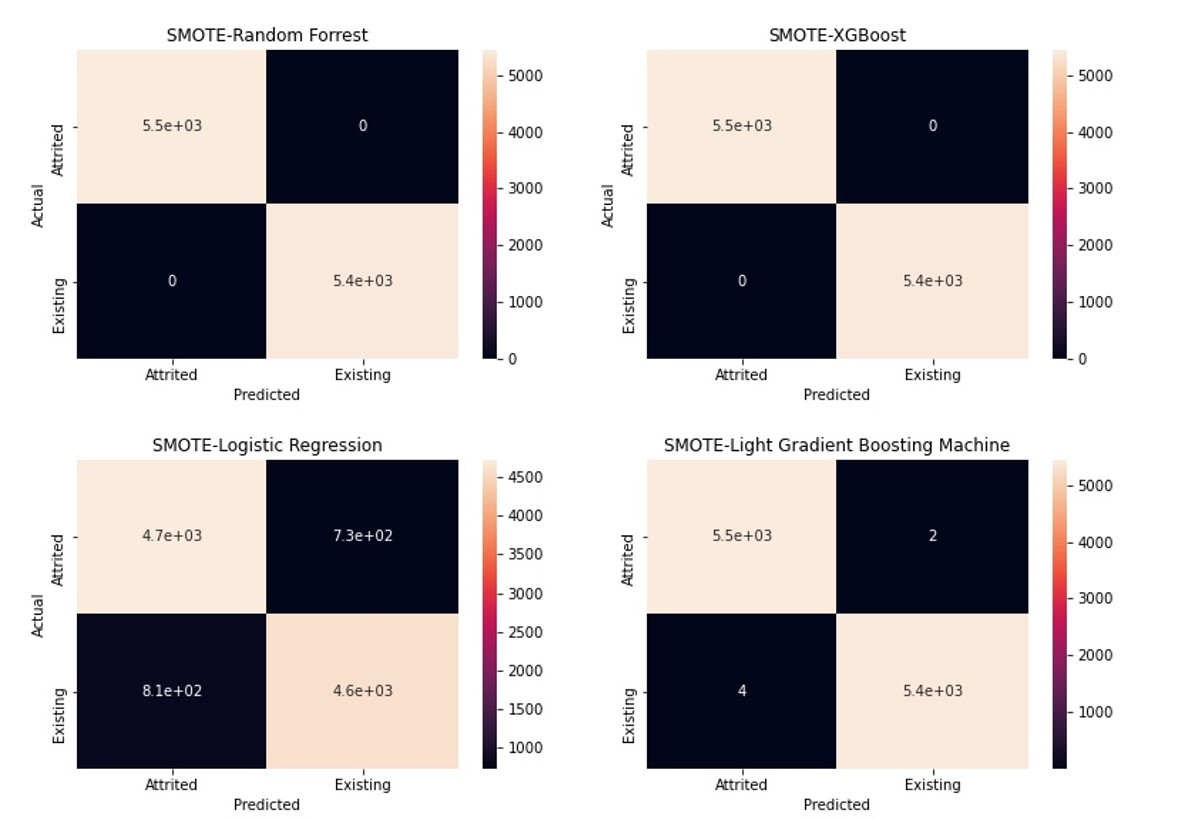
\includegraphics[scale=0.6]{figure/ML with SMOTE.jpg}
    \caption{Confusion Matrix: Machine Learning SMOTEd Data}
    \label{fig:MLSmotedCM}
\end{figure}

\subsection{Neural Network Chronological Accuracy \& Loss and Confusion Matrix}
\subsubsection{Long Neural Network}
It can be seen that the SMOTEd data performed better with smaller fluctuation and also better distribution of confusion matrix.
\begin{figure}[H]
    \centering
    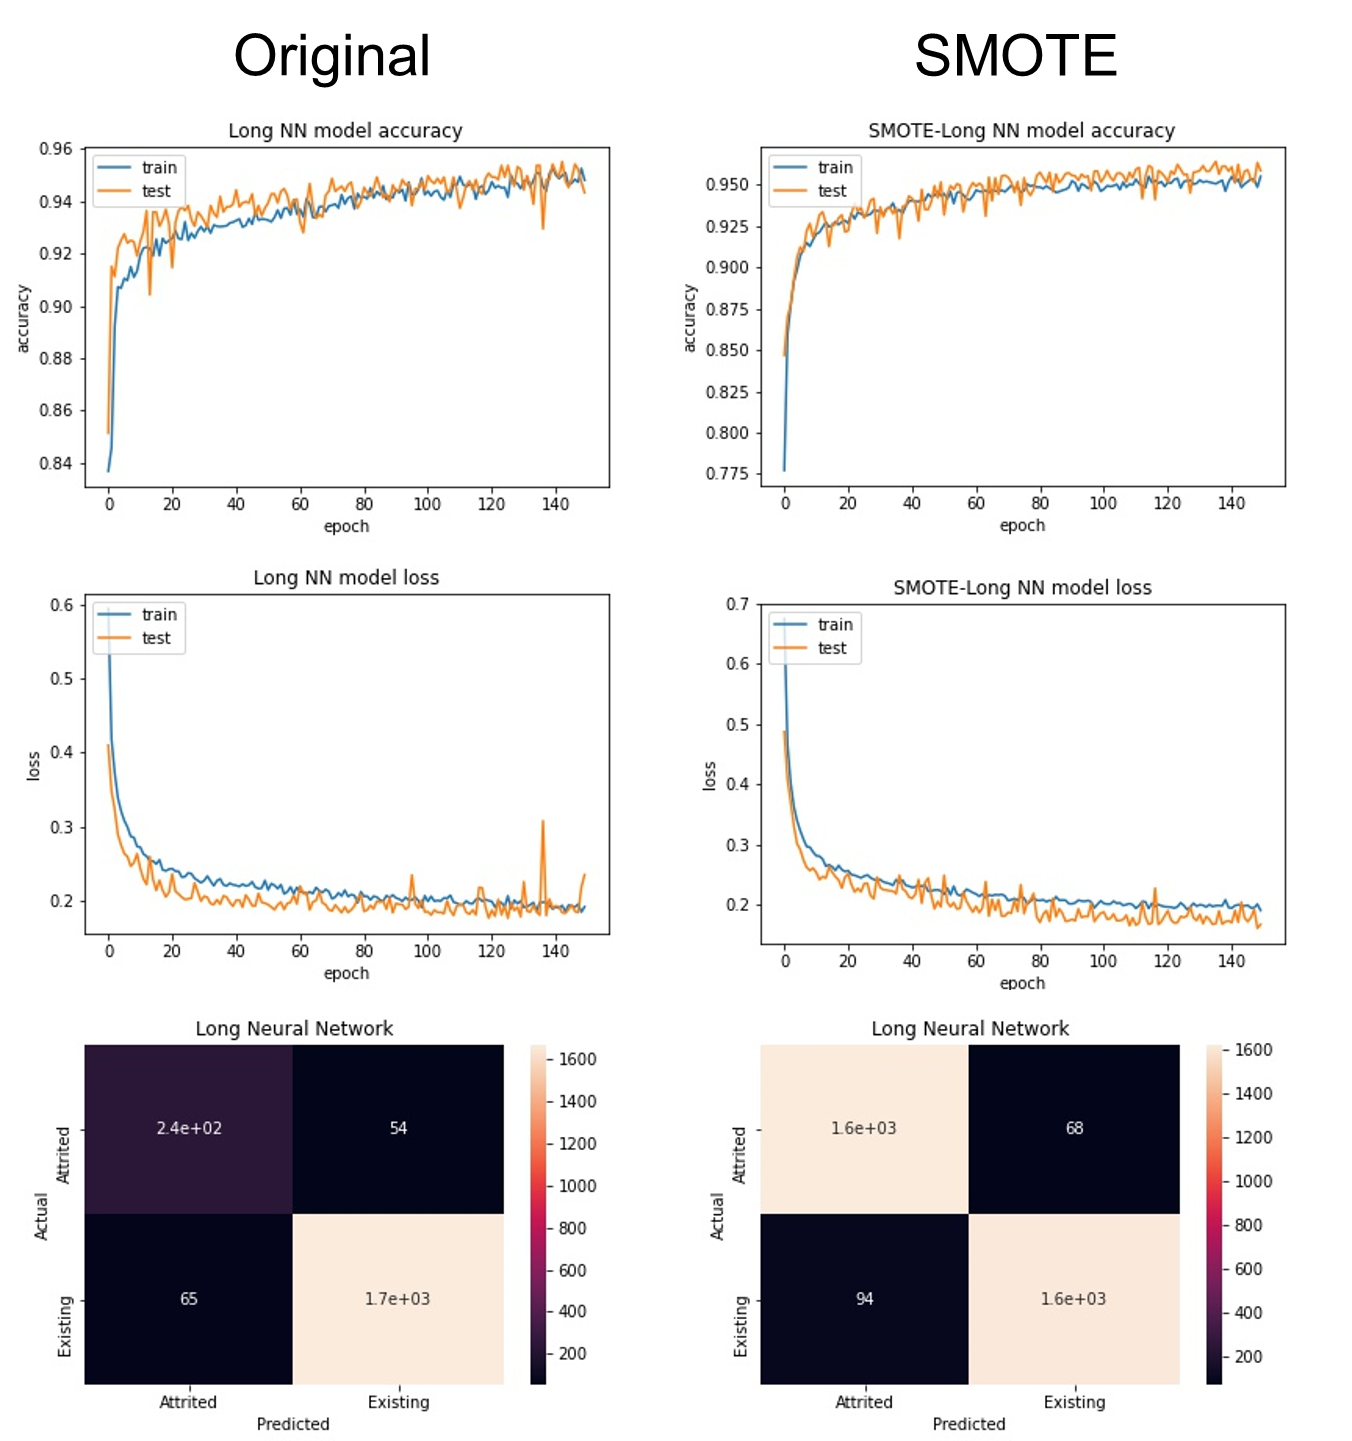
\includegraphics[scale=0.6]{figure/LONG NN SUMMAR.png}
    \caption{Long Neural Network}
    \label{fig:LNNSummary}
\end{figure}

\subsubsection{Wide Neural Network}
It can be seen that the SMOTEd data performed better with smaller fluctuation and also better distribution of confusion matrix.
\begin{figure}[H]
    \centering
    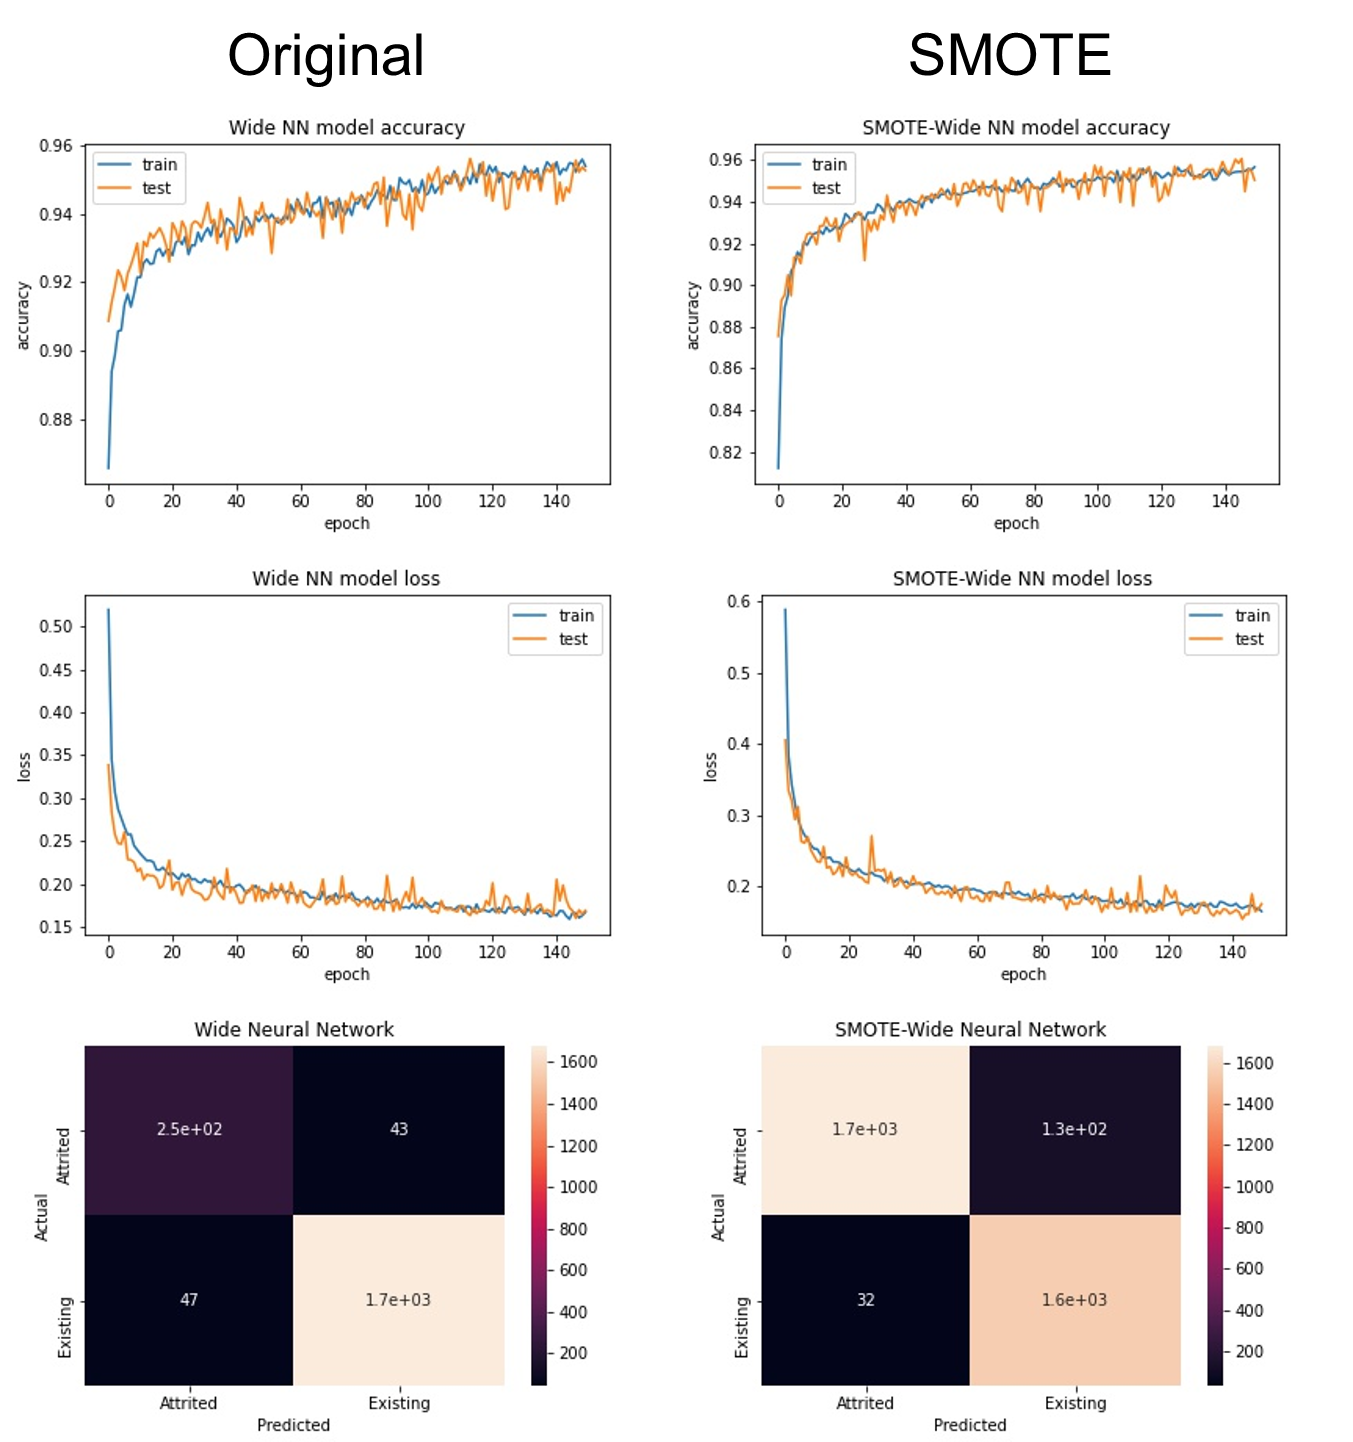
\includegraphics[scale=0.6]{figure/WIDE NN SUMMAR.png}
    \caption{Wide Neural Network}
    \label{fig:WBBSynnary}
\end{figure}

\subsection{Machine Learning and Deep Learning Accuracy, F1 Score and Recall}
It can be seen that models trained with SMOTEd data are performing really well due to the absence of training frequency bias. Wide Neural Network can perform really well with high F1 score and Recall. LGBM Machine Learning Also performing excellently with overall 98\% scores. Perfect!\\
Cross Validated accuracy are also very close to the Accuracy by test data, which is a good sign that the model are not over-fitted! Excellent!
\begin{figure}[H]
    \centering
    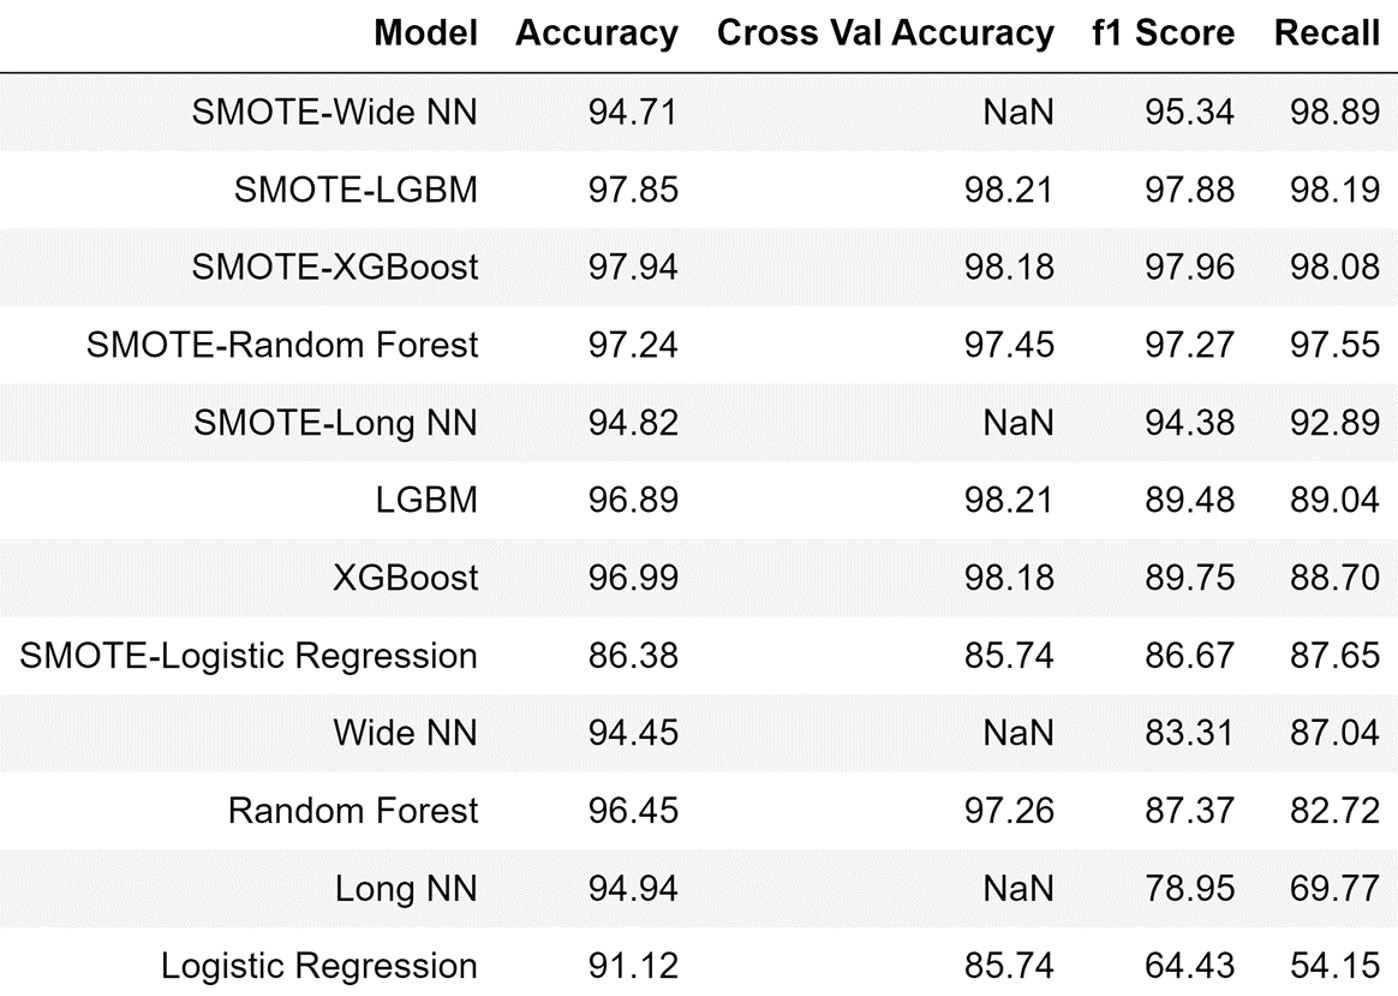
\includegraphics[scale=0.6]{figure/Summary.jpg}
    \caption{Summary}
    \label{fig:summary}
\end{figure}
\subsection{Justification}
Confusion Matrix can tell us directly the proportion of the Predicted and Actual data, whether there are any Falsely classified data.
Accuracy parameters can tell us how well the Prediction matched with the Actual value. 
F1 and Recall can tell us how well the classification of the True and Predicted. 
The better the values reach 100\% the better the model is.
\section{Model Deployment}
The machine Learning models were deployed and saved in "sav" files as follow:\\
\textbf{Original}
\begin{center}
\begin{tabular}{ |c|c|c| } 
 \hline
 \hline
 \textbf{Machines} & \textbf{Name} & \textbf{Filename} \\ 
 \hline
 \hline
 Random Forest & rf & rf.sav \\ 
 \hline
 Logistic Regression & lr & lr.sav \\ 
 \hline
 XGBoost & xgb & xgb.sav \\ 
 \hline
 Light GBM & lgbm & lgbm.sav \\ 
 \hline
 \hline
\end{tabular}
\end{center}
\textbf{SMOTEd}
\begin{center}
\begin{tabular}{ |c|c|c| } 
 \hline
 \hline
 \textbf{Machines} & \textbf{Name} & \textbf{Filename} \\ 
 \hline
 \hline
 Random Forest & rfsm & rfsm.sav \\ 
 \hline
 Logistic Regression & lrsm & lrsm.sav \\ 
 \hline
 XGBoost & xgbsm & xgbsm.sav \\ 
 \hline
 Light GBM & lgbmsm & lgbmsm.sav \\ 
 \hline
 \hline
\end{tabular}
\end{center}

The deep learning models were deployed and saved in a "json" files and the weights were saved in "h5" formats, as follow:

\begin{center}
\begin{tabular}{ |c|c|c|c| } 
 \hline
 \hline
 \textbf{Machines} & \textbf{Name} & \textbf{model} & \textbf{weight}\\ 
 \hline
 \hline
 Long NN & nn\_model & nn\_model.json & nn\_model.h5 \\ 
 \hline
 Wide NN & nn\_model2 & nn\_model2.json & nn\_model2.h5 \\ 
 \hline
 SMOTEd-Long NN & nn\_model1sm & nn\_model1sm.json & nn\_model1sm.h5 \\ 
 \hline
 SMOTEd-Wide NN & nn\_model2sm & nn\_model2sm.json & nn\_model2sm.h5 \\ 
 \hline
 \hline
\end{tabular}
\end{center}

\subsection{Justification}
The models were saved in files as it will be easier to distributed and saved in a local repository or GitHub. They can be easily loaded and used should there are any new upcoming data. \\
Jupyter Notebook file the "*.ipynb" file is also saved, but even without it, with the help of this ADD, the next data scientist will be able to easily replicate the analysis and model building process.

\section{Summary}
The model has been successfully built with LGBM is the best performing Machine Learning and Wide Neural Network as the best Deep Learning algorithm. \\
SMOTE tool is essential to synthesis unequal data, and to get a better training and remove bias.
The worst is Logistic Regression. Do not use it!

\end{document}
